\setchapterimage[2cm]{../images/header-methods.jpg}
%\setchapterpreamble[u]{\margintoc}
\chapter{Computational methods and specifications}
\labch{methods}

\section{Methods and techniques}

Throughout this work, many different computational methods and techniques were employed in order to carry out a diverse set of studies.
Some of them, the ones that are the most relevant to the flow of the work, are specifically explained and developed in detail in their own sections.
Others, however, are deemed to be more of a general character, already well known within the field, or unimportant for the understanding of the main ideas of this thesis.
This section is meant to serve as an overview of the methodology, specifications and theory behind the whole study, and also to provide explanations for that less special set of techniques.
This part may be skimmed and consulted at a later time, or even skipped entirely, as the rest of the work is presented in such a way that can be followed without deep knowledge of the subjects that are explained here.

\subsection{Calculation level}
All of the electronic structure calculations were performed using Density Functional Theory (DFT) in the Kohn-Sham formulation.
Specifically, the functional of choice was Minnesota's M06-2X.\sidecite{truhlar08}
M06-2X is a highly parametrized hybrid meta-GGA functional that features a \SI{54}{\percent} of Hartree-Fock exchange.
It was chosen because it has been extensively trained to perform well in a variety of contexts that include thermochemistry, the study of non covalent interactions, and vibrational and electronic spectroscopy, appearing in numerous publications in the bibliography supporting its effectiveness.\cite{head16,vidalvidal17,vidalvidal17-2,vidalvidal18,sert14,eizig15,coccia17}
While the molecules discussed in the work are novel and have not been previously characterized, it's expected that their chemistry and their spectroscopic behavior aren't out of the ordinary.
Therefore, it should be possible to describe them properly and efficiently with such a functional.

As for the basis functions, the set of choice was Weigend and Ahlrichs' def2-SVP.\sidecite{ahlrichs05}
def2-SVP is of split valence set and includes polarization functions, but is overall a fairly small set.
However, it has been deemed sufficiently extense to obtain accurate geometry optimizations, and qualitatively good energies and spectra.

Considering the size of the systems of the study, the large amount of planned computations, the available computational resources, and the actual accuracy needs of the project, the M06-2X and def2-SVP calculation level was considered appropriate.

\subsection{Geometry optimization}
The optimization of the geometry of a molecule is a crucial part of any computational modeling.
At its core, it's a process where the geometry of a system gets iteratively modified (and its energy gets calculated at each step) with the aim of reaching a stationary point on its potential energy surface.
In the case of this work, these optimizations are always minimizations as we just look for energy minima.
In Gaussian09,\cite{gaussian09} our electronic structure computation software of choice, these calculations are carried out using the Berny algorithm in its GEDIIS\sidecite{li06} implementation.

\subsection{Magnetic shielding computation}
Nuclear magnetic resonance type calculations, namely the computation of the magnetic shielding in the Nucleus-Independent Chemical Shift study in \refsec{nics}, were carried out using the GIAO method.
GIAO stands for gauge-including atomic orbital.
It solves what is often referred to as \q{the gauge problem}, which can be defined as an error that arises when doing calculations with a magnetic perturbation while having the atomic orbital basis functions depend on position.\sidecite{magyarfalvi11}
Magnetic perturbations usually affect the atomic orbital set of a molecule as rotations.
Atomic orbitals located near to the axis of the rotation won't suffer from this error, as their basis sets should still be able to properly describe the perturbed wave function.
However, as the distance to the axis of rotation increases, the linear translation due to a rotation gets larger, and the description of the atomic orbitals gets progressively worse.
The GIAO method solves this problem by using sets of atomic basis functions that depend explicitly on the magnetic field.

GIAO calculations have been successful in describing the magnetic shielding of a variety of large nuclei in optimized and isolated large molecules.\sidecite{yuksek08} Therefore, it has been considered as an appropriate way of computing the absolute magnetic shieldings needed in this work.

\subsection{Electronic transition study}
\labsec{electronic-transition-study}
The prediction of ultraviolet-visible (UV-vis) spectra, a result of electronic transitions within a molecule, requires the computation of the energies of its electronically excited excited states.
As the electromagnetic waves responsible for such excitations have a time-dependent nature, in this work this is achieved through the application of time-dependent DFT.\sidecite{runge84,adamo13}

\subsection{Vibrational analysis}
Any given non linear molecule with $N$ atoms has 6 translational and rotational normal modes, and $3N-6$ vibrational ones.
Vibrational normal modes are orthogonal, that is, they're vibrational motions that are independent and don't cause movement to the other normal modes.

The frequencies of these modes are calculated through the following procedure.\sidecite{ochterski99}
\fix{First, a}
\blindtext[2]

\subsubsection{Normal mode calculation and decomposition}
\labsec{intmodes-methods}
By translating the cartesian displacements that result from the frequency calculations into redundant internal coordinates, it's possible to identify which of the atoms of the molecule or system are the most involved in a particular vibrational mode.
Having the vibrations expressed in such a way is useful in automating the analysis of modes.
In this work, this is used to classify the vibrational modes of a dimer.
Each individual vibration within the mode is classified by whether it belongs to molecule A, to molecule B, or is a mixture of the two.
Thanks to this calculation, the modes can be filtered by their percentage of A, B or mixed vibrations.
This idea is further explored and applied in \refsec{heatmaps}.

\subsection{Raman spectroscopy}
Raman spectroscopy is a technique that allows for the detection of those vibrational normal modes that affect the polarizability of a molecule (i.e. the ease with which its electron cloud can be distorted).
This kind of vibrational transitions are tied to a physical phenomenon known as Raman or inelastic scattering.
For an inelastic scattering event to happen, a photon has to excite a molecule and get it to a virtual energy state before being emitted.
After this, the photon has either a lower or a higher energy, and the molecule ends up in a different vibrational or rotational state due to the energy exchange between them.

\fix{Explain how Raman modes are identified and how are their intensities calculated.}
\blindtext

\subsubsection{Resonance Raman}
\labsec{rr-methods}
The regular Raman effect is usually very weak, as the probability of Raman scattering occurring is extremely low.\sidenote{Only about 1 in every \num{1e7} photons results in inelastic scattering}

\begin{marginfigure}
    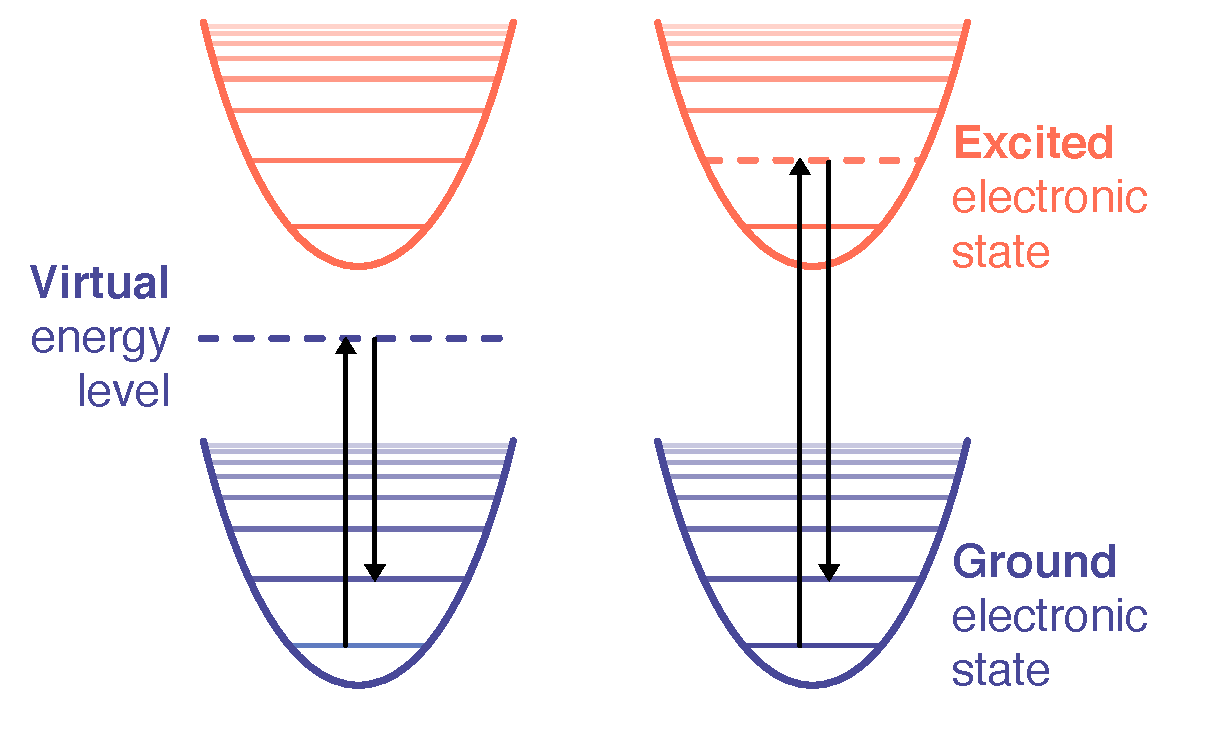
\includegraphics{raman-rr-comparison}
    \caption[Standard and resonance Raman excitations]{Standard and resonance Raman excitations}
    \labfig{raman-rr-comparison}
\end{marginfigure}

Resonance Raman (RR) spectroscopy is a variation of Raman in which the intensities are greatly amplified.
This technique relies in the usage of a carefully selected laser wavelength to perform the measurement: if it's close enough to an electronic transition, the scattering effect, and therefore the intensity of the measured Raman peaks, can increase by several orders of magnitude.
In regular Raman scattering, the energy that the molecule absorbs from the photon just makes it reach a virtual energy level before returning to a different rotational or vibrational state.
By using photons that have the same energy as electronic transitions, however, the molecule reaches a real excited electronic state as shown in \reffig{raman-rr-comparison}.
This excited state has a different geometry, and that affects the polarizability of the molecule and increases the magnitude of the subsequent Raman signal.\sidecite{hirakawa75}

\fix{Explain how it's calculated using CPHF!}
\blindtext

\subsubsection{Surface-enhanced Raman spectroscopy and surface interactions}
Surface-enhance Raman spectroscopy (SERS) is a variation of Raman spectroscopy that explores the large enhancements in intensity that the Raman signals of a molecule may experience when interacting with a surface.
While such effect was originally observed in roughened silver and is usually studied using metal surfaces and clusters, it has also been found in non-metal nanostructures and surface-like molecules, which will be referred to as \q{SERS substrates}.
The nature of this effect has been related to resonance.
Specifically, it's been said that it draws upon three different kinds: surface plasmon resonance, charge-transfer resonance, and molecular resonance.\sidecite{lombardi08}
The first of these effects, surface plasmon resonance, is defined as the coherence of the oscillation of the conduction electrons of the substrate\marginnote{Such as the free flowing electrons in a metal cluster, or the electron cloud of a large conjugated covalent system such as graphene} with an external exciting electromagnetic radiation.
Charge-transfer resonance may be present when there is a significant transfer of electron density between the substrate and the molecule.
Finally, molecular resonance may appear too as a property almost exclusive to the molecule, but can still have a significant contribution to the total effect.

The main focus of this work, however, is Resonance Raman.
The adsorption of the molecule to a substrate makes it benefit from SERS effects, but it shares importance with its other purpose: shifting the UV-vis absorption range.
Adhering a molecule that absorbs short wavelengths to a substrate that absorbs long ones may result in a complex that has a range of absorption that's higher than that of the molecule alone.
Since real-life laser devices for Raman spectroscopy can get rare, expensive and energetic to the point of being destructive as the wavelength gets shorter, it's desired to achieve such effects.
For these reasons, while SERS is an interesting technique that certainly plays a part in the results achieved in this work, we don't delve too deep into the explanation of its nature.

\subsection{Spectra envelope calculation}
\labsec{spectra-envelope-calculation}

\begin{margintable}
    \centering
    \caption[Raman activity of STX]{Raman activity for each vibrational mode of STX}
    \begin{tabular}{@{}c
                       S[table-format=1.4]
                       S[table-format=1.4]@{}}
        \toprule
        {Mode} & {$\tilde{\nu}$ \si{\per\cm}} & {Ram. act.} \\
        \midrule
        1 & 0.0917 & 0.0236 \\
        2 & 0.9542 & 1.9687 \\
        3 & 0.8552 & 1.2691 \\
        4 & 1.7897 & 3.3270 \\
        \multicolumn{3}{c}{{\ldots}}
    \end{tabular}
    \labtab{oscillator-strengths}
\end{margintable}

This work deals with two types of spectra: electronic and vibrational.
Computational chemistry software is able to predict spectroscopic values such as electronic transition energies, vibrational mode wave numbers, Raman activities and oscillator strengths.
However, to get from those numbers to the familiar bands and peaks that are characteristic of experimental spectra, a few extra steps are involved.
This additional representation procedure will be exemplified by plotting both kinds of spectra for the saxitoxin (STX) molecule.

We start from the list of vibrational normal modes that results from a Raman calculation.
Then, their vibrational frequencies in the form of wave numbers as well as their corresponding Raman activity values are extracted using a custom script.
Plotting these values directly as vertical lines along the wave number range results in \reffig{without-envelope}.

\begin{figure}
    \centering
    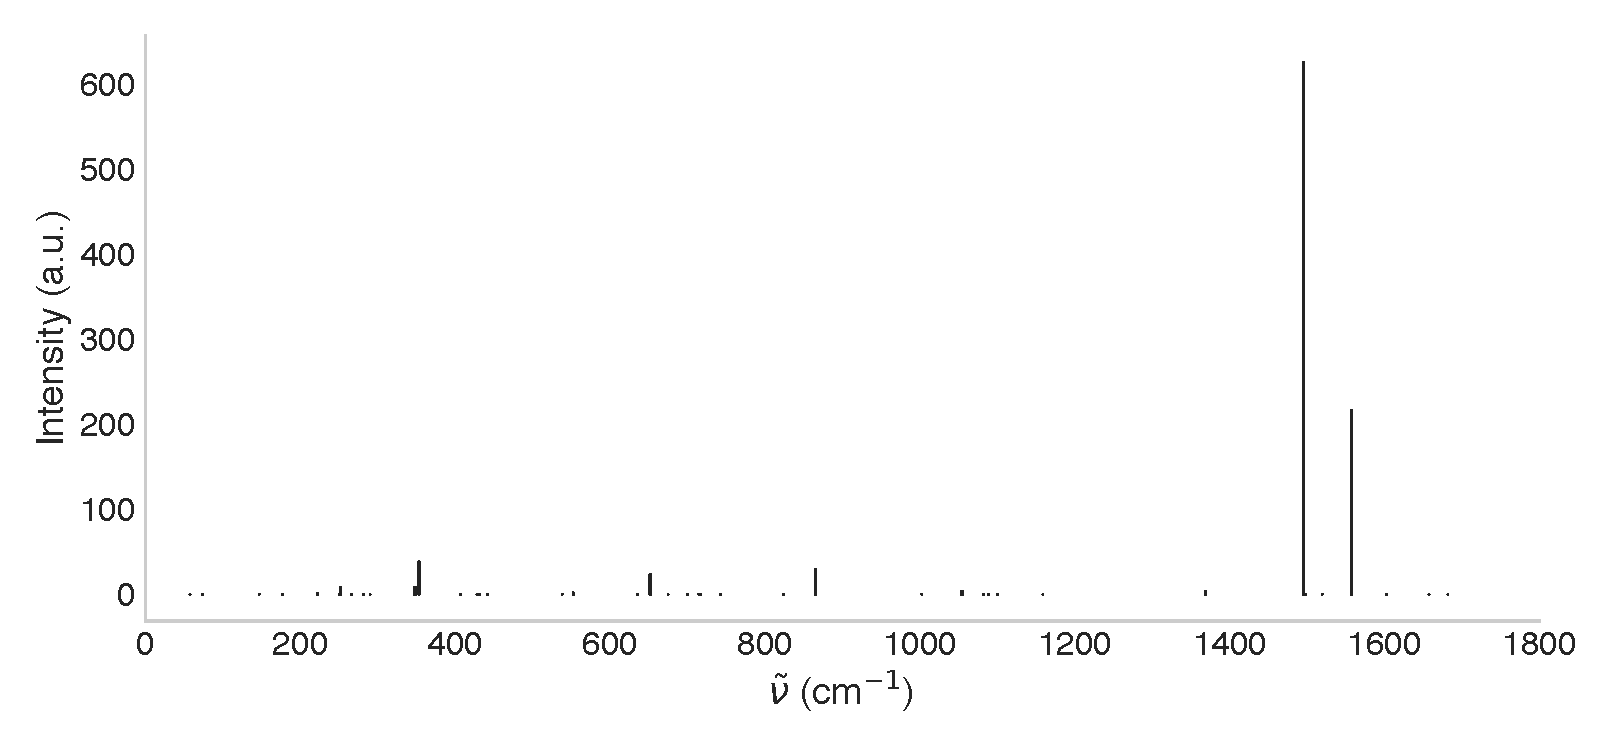
\includegraphics{without-envelope}
    \caption[Raman spectrum as simple peaks]{Raman spectrum of STX using a simple peak representation}
    \labfig{without-envelope}
\end{figure}

While such a graph could still be useful to display and compare the intensities of the vibrational modes, it could be harder to compare to real experimental spectra.
In order to make our theoretical spectra look more realistic, then, an envelope line is added.
This is done by replacing each of the simple vertical lines by Gaussian functions.
These functions are designed so that they are as tall as the intensity of the peak that they're representing.
They are evaluated at the full range of frequencies, and linearly combined forming a continuous curve that smoothly wraps all of the peaks.

In the case of Raman spectra, the value of each of the Gaussians at a certain wave number value is calculated following \refeq{raman-envelope}.

\begin{equation}
    \labeq{raman-envelope}
    I_i (\tilde{\nu}) = I_i^\textit{max}e^{-\left(\frac{\tilde{\nu} - \tilde{\nu}_i}{\sigma}\right)^2}
\end{equation}

The value of $\sigma$, which is the full width at half maximum of each curve, is set arbitrarily at \SI{4}{\per\cm}.
The same STX Raman spectrum, plotted after computing this set of equations, is displayed in \reffig{with-envelope}.

\begin{figure}
    \centering
    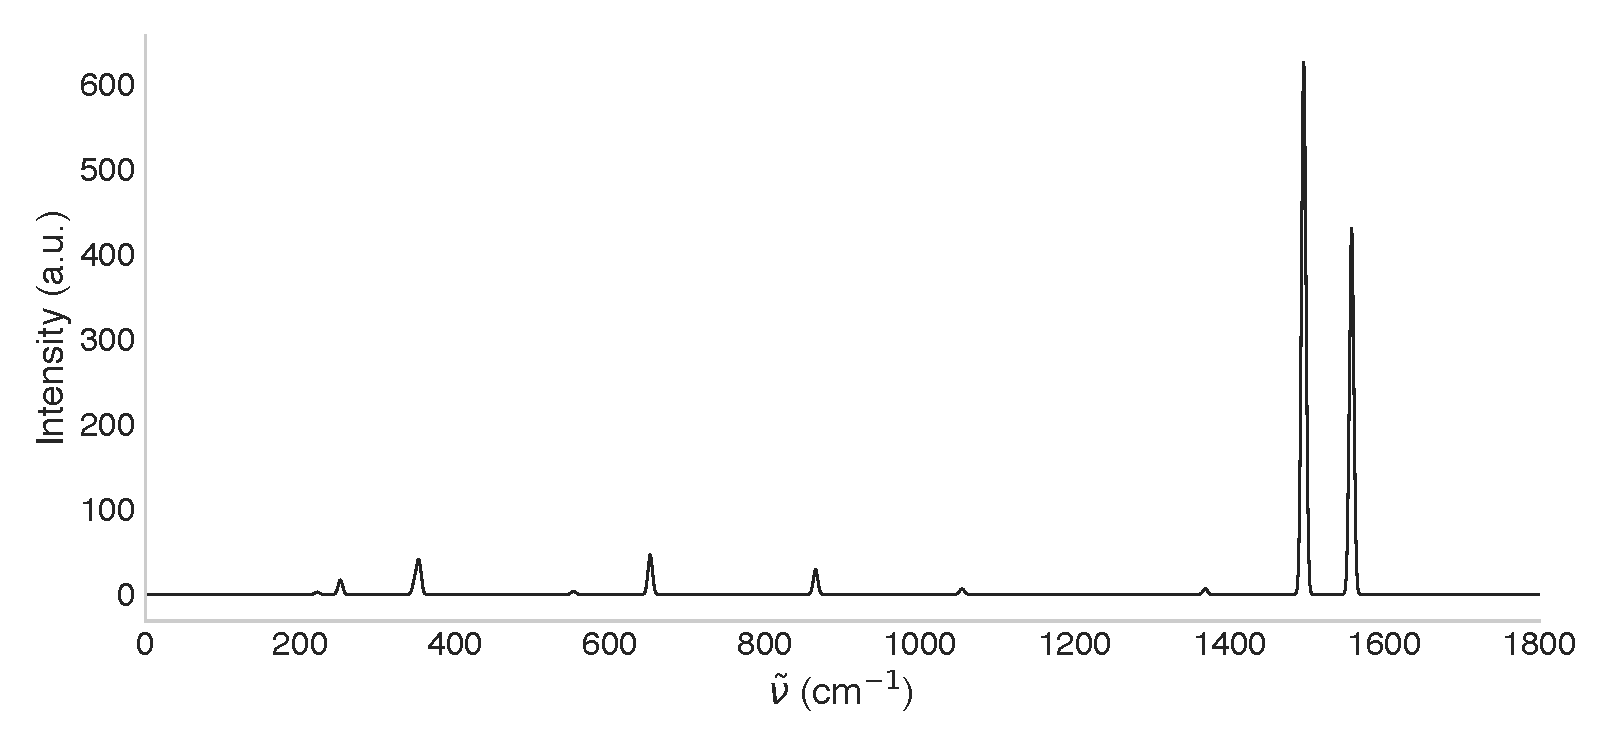
\includegraphics{with-envelope}
    \caption[Raman spectrum with Gaussian envelope]{Raman spectrum of STX using an envelope of Gaussian functions}
    \labfig{with-envelope}
\end{figure}

As for the electronic spectra, the procedure is quite similar.
In this case, the values to be plotted are the energies of the electronic transitions in the form of wavelengths, as well as their corresponding oscillator strengths.
Similarly to before, an envelope curve is created by calculating as many Gaussian functions as there are transitions, but with a slightly different formula as displayed in \refeq{uv-envelope}.

\begin{equation}
    \labeq{uv-envelope}
    \varepsilon_i (\lambda)) = \num{1.306297e8} \frac{f_i}{\sigma} e^{-\left(\frac{1/\lambda - 1/\lambda_i}{\sigma}\right)^2}
\end{equation}

Here, $\lambda_i$ and $f_i$ are the wavelength and oscillator strength of each transition. The constant before the exponential\marginnote{
\begin{equation}
    \labeq{uv-constant}
    \frac{\sqrt{\pi} e^2 N}{1000 \ln(10) c^2 m_e} = \num{1.306297e8}
\end{equation}
Where $e$ and $m_e$ are the charge and mass of the electron, $N$ is Avogadro's number, and $c$ is the speed of light
} (see \refeq{uv-constant}) is a conversion factor that is added in order to achieve the right units for the intensity $\varepsilon$, which should be \si{\litre\per\mole\per\cm}.
A value of \SI{0.4}{\eV} was chosen for $\sigma$.
For the case of STX, the spectrum that results from combining the Gaussian band shapes for the 50 most intense electronic transitions is shown in \reffig{uv-envelope}

\begin{figure}
    \centering
    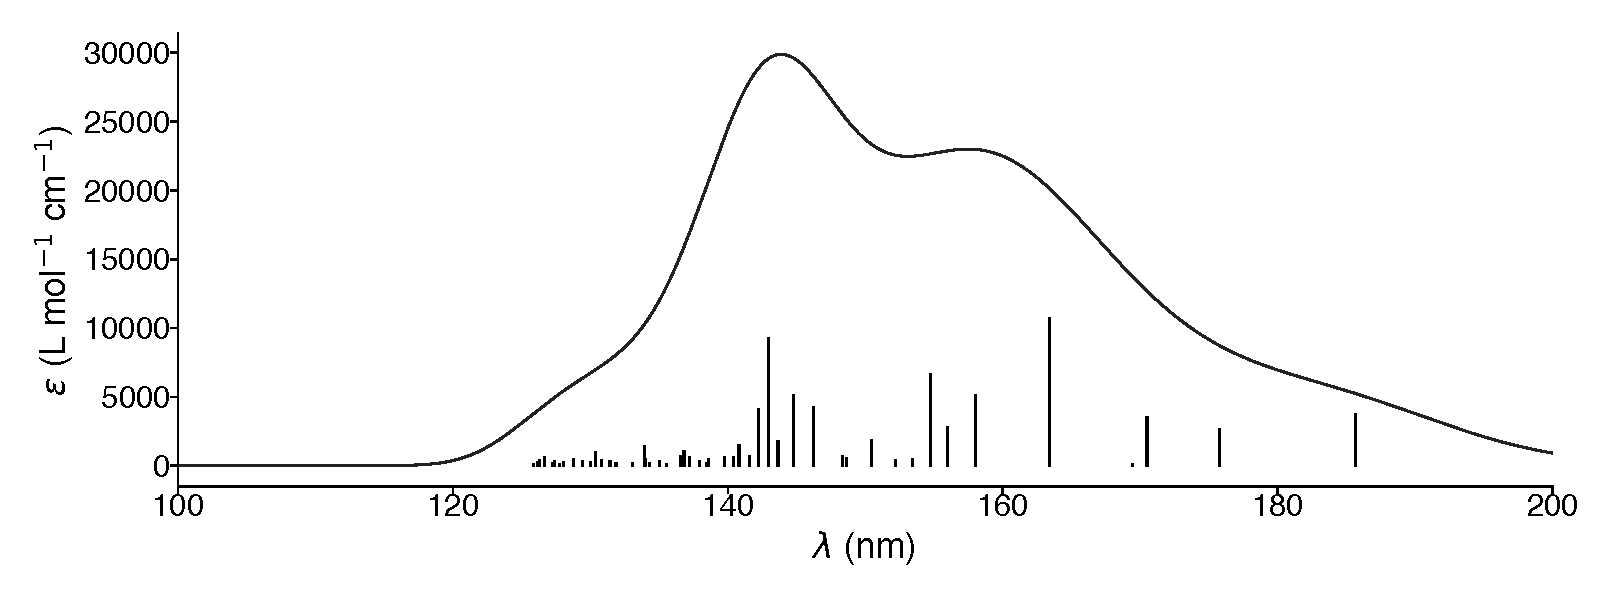
\includegraphics{uv-envelope}
    \caption[Electronic spectrum with Gaussian envelopes]{Electronic spectrum of STX using an envelope of Gaussian functions}
    \labfig{uv-envelope}
\end{figure}


\section{Software}

The software used to perform all of the calculations is summarized in \reftab{computational-techinques}

\begin{table*}[h]
    \centering
    \caption[Overview of techniques, level and software]{Overview of the computational techniques, calculation level and software that were used in this work}
    \labtab{computational-techinques}
    \begin{tabular}{@{}llllll@{}}
        \toprule
        Calculation & Technique & Spec. & Functional & Basis set & Software \\
        \midrule
        Geometry optimization                   & DFT       & GEDIIS    & M06-2X & def2SVP & Gaussian09 \\
        Vibrational analysis                    & DFT       &           & M06-2X & def2SVP & Gaussian09 \\
        Raman activity                          & DFT       &           & M06-2X & def2SVP & Gaussian09 \\
        Resonance Raman activity                & DFT       & CPHF      & M06-2X & def2SVP & Gaussian09 \\
        Electronic transition calculation       & TD-DFT    &           & M06-2X & def2SVP & Gaussian09 \\
        Magnetic shielding calculation          & DFT       & GIAO      & b3lyp  & 6-31G*  & Gaussian09 \\
        Surface generation                      &           &           & & & nics.py \\
        \bottomrule
    \end{tabular}
\end{table*}


\section{Hardware}
All of the electronic structure calculations were performed using either the Centro de Supercomputación de Galicia's (CESGA) infrastructures, or the propietary cluster of the S3 research group.

CESGA's supercomputer, FinisTerrae-II (FTII), is a Bull ATOS bullx machines that features \num{320} computation nodes, \num{7712} cores, \SI{44544}{\giga\byte} of RAM, and \SI{750000}{\giga\byte} of storage capacity.
All of the calculations carried out at FTII were performed in standard nodes, utilizing \num{12} cores at a time, and \SI{60}{\giga\byte} of RAM.
These nodes include each 2 Intel\textregistered Xeon\textregistered E5-2630 v3 \SI{2.50}{\giga\hertz} processors with \num{24} cores total, and \SI{128}{\giga\byte} of RAM.

S3's cluster is composed of nodes that feature \num{16} cores running on Intel\textregistered Xeon\textregistered E5-2630 v3 \SI{2.40}{\giga\hertz} processors, and \SI{64}{\giga\byte} of RAM.

Smaller calculations such as input file generation, output parsing, surface estimation, graph representation... were carried out in the author's personal computer.
